\chapter{Planificació}

L'inici del projecte es pot considerar el 5 de febrer de 2024, que va ser quan es va contactar per primera vegada amb el tutor. La fi es pot considerar la data d'entrega de la memòria, el 4 de setembre de 2024.

Les etapes que s'han seguit, tal com s'estipula al \autoref{cap:5}, es detallen a continuació. Cada etapa comença quan finalitza l'anterior, i en totes es documenta el procés. El seguent diagrama es pot mirar com a resum: \autoref{fig:DiagramaGant}

\section{Escriure la proposta del TFG}

La primera etapa es va desenvolupar fins al 16 de febrer, dia en què es va presentar la proposta del TFG a la comissió de TFG.Aquesta fase va consistir a explicar al tutor diverses idees per al TFG, relacionades amb la voluntat de desenvolupar un joc senzill persistent i consolidar-ho en un treball sobre infraestructura al núvol, per a poder valorar la capacitat d'aquestes estructures per suportar grans càrregues de treball.Després de treballar sobre aquestes idees principals, es va arribar a la idea plasmada en aquest treball: fer una anàlisi de la infraestructura actual disponible per a un usuari qualsevol i aplicar-hi estrès per poder avaluar el rendiment.

\newpage
\section{Buscar el servidor del joc}

Durant aquesta etapa, que va finalitzar el 6 de març, l'objectiu va ser escollir un bon candidat de servidor sobre el qual elaborar l'anàlisi i les proves d'estrès.La idea inicial de desenvolupar un joc senzill com a part del treball va ser ràpidament descartada en veure que crear-ne un que complís amb els requisits de ser fàcilment compatible amb les eines d'estrès, que tingués certa complexitat i funcionés a les dues màquines, hauria deixat poc temps per fer un anàlisi rellevant al títol i objectiu principal del treball.Així doncs, aquesta etapa va consistir en l'exploració de servidors de backend de videojocs que complissin aquests requisits a la plataforma \textit{GitHub}.


\section{Instal·lació dels servidors i recerca sobre tests de càrrega}

La següent etapa, que va durar fins al 15 de març, va consistir en aconseguir les dues màquines en les quals s'instal·larien els servidors, instal·lar el servidor en ambdues màquines, i començar a buscar i provar diferents programes o llenguatges per fer els tests de càrrega, amb l'objectiu d'estressar els servidors i obtenir dades interessants sobre les seves capacitats.

\section{Desenvolupament dels tests de càrrega}

Aquesta etapa, que finalitza el 3 de juliol, va consistir en la selecció de l'eina open-source \textit{k6}, en la qual es van escriure els tests de càrrega.

\section{Redacció del treball}

L'etapa final ha consistit en la recopilació de tota la documentació escrita en les etapes anteriors i la  finalització de la redacció de la memòria i el resum redactat durant tot el projecte.


\begin{figure}[!htbp]
    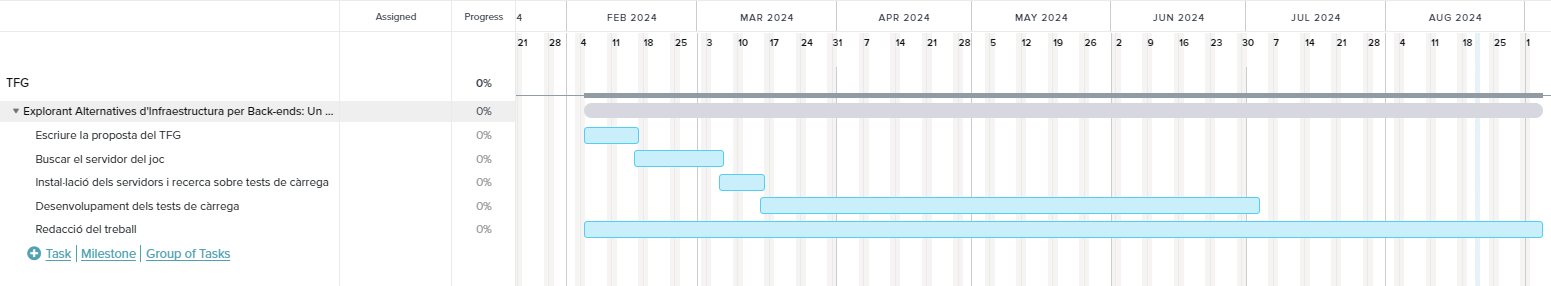
\includegraphics[scale=0.30]{Imatges/Diagrama de Gantt.png}
    \label{fig:DiagramaGant}
    \caption{Diagrama de Gantt planificació realitzada}
    
\end{figure}
